\documentclass[12pt]{article}

\usepackage{amsmath, amssymb}
\usepackage[margin=1in]{geometry}
\usepackage{helvet}
\usepackage{tikz}
% \usepackage{figure}
\renewcommand{\familydefault}{\sfdefault}

\begin{document}
\def\assignment{Homework 01}

\pagenumbering{gobble}
\noindent{\large COSC 4765 \hfill Name: \underline{Jacob Tuttle} \\ Computer Security}
\begin{center}
    {\Large \assignment} \\ \textbf{\today}
\end{center}


\question{1. Large Scale Access Control}

One of the largest limitation to using matrix based access control for a large organization is managing to find your way to the correct entry quickly. Even using some efficient sorting and searching system will require an increasing number of actions as the number of users grows into the hundreds of thousands. On top of that, storing all of that data, much of it repeated since there is a limited number of possible access right levels.

In order to build a data structure that allows for quick retrieval, let's try to leverage a hash table to do it. We can use the usernames to reference the users in a lockup table that points to the subset of possible rights they have access to. \\

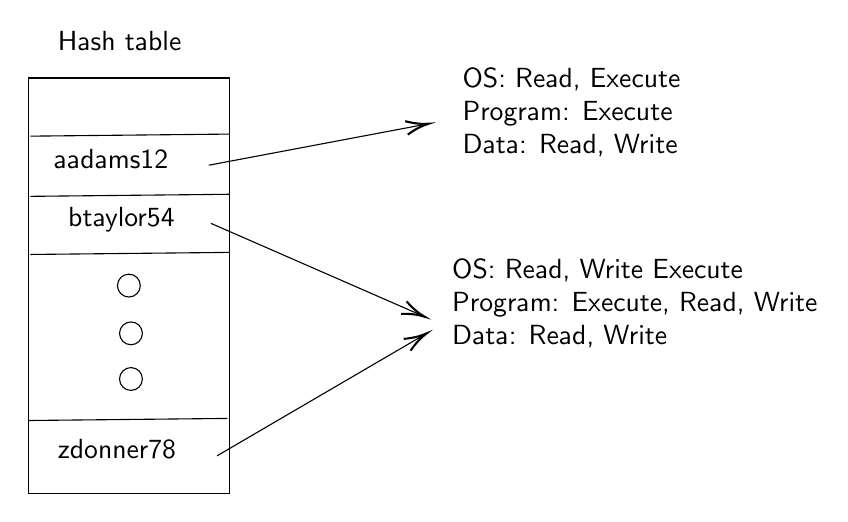
\begin{tikzpicture}[x=0.75pt,y=0.75pt,yscale=-1,xscale=1]
    %uncomment if require: \path (0,300); %set diagram left start at 0, and has height of 300

    %Shape: Rectangle [id:dp9165563207385413] 
    \draw   (30,42) -- (127,42) -- (127,242) -- (30,242) -- cycle ;
    %Straight Lines [id:da0759341585311688] 
    \draw    (117,84) -- (221.03,64.37) ;
    \draw [shift={(223,64)}, rotate = 529.3199999999999] [color={rgb, 255:red, 0; green, 0; blue, 0 }  ][line width=0.75]    (10.93,-3.29) .. controls (6.95,-1.4) and (3.31,-0.3) .. (0,0) .. controls (3.31,0.3) and (6.95,1.4) .. (10.93,3.29)   ;
    %Straight Lines [id:da6125316607464432] 
    \draw    (31,70) -- (127,69) ;
    %Straight Lines [id:da6222430940564477] 
    \draw    (31,99) -- (127,98) ;
    %Straight Lines [id:da4720191386501048] 
    \draw    (31,127) -- (127,126) ;
    %Straight Lines [id:da550449578722363] 
    \draw    (30,207) -- (126,206) ;
    %Shape: Ellipse [id:dp0388578248616509] 
    \draw   (73,142) .. controls (73,138.96) and (75.46,136.5) .. (78.5,136.5) .. controls (81.54,136.5) and (84,138.96) .. (84,142) .. controls (84,145.04) and (81.54,147.5) .. (78.5,147.5) .. controls (75.46,147.5) and (73,145.04) .. (73,142) -- cycle ;
    %Shape: Ellipse [id:dp9914541781124333] 
    \draw   (74,165) .. controls (74,161.96) and (76.46,159.5) .. (79.5,159.5) .. controls (82.54,159.5) and (85,161.96) .. (85,165) .. controls (85,168.04) and (82.54,170.5) .. (79.5,170.5) .. controls (76.46,170.5) and (74,168.04) .. (74,165) -- cycle ;
    %Shape: Ellipse [id:dp1296877334676496] 
    \draw   (74,187) .. controls (74,183.96) and (76.46,181.5) .. (79.5,181.5) .. controls (82.54,181.5) and (85,183.96) .. (85,187) .. controls (85,190.04) and (82.54,192.5) .. (79.5,192.5) .. controls (76.46,192.5) and (74,190.04) .. (74,187) -- cycle ;
    %Straight Lines [id:da1399761729430522] 
    \draw    (118,112) -- (219.17,156.2) ;
    \draw [shift={(221,157)}, rotate = 203.6] [color={rgb, 255:red, 0; green, 0; blue, 0 }  ][line width=0.75]    (10.93,-3.29) .. controls (6.95,-1.4) and (3.31,-0.3) .. (0,0) .. controls (3.31,0.3) and (6.95,1.4) .. (10.93,3.29)   ;
    %Straight Lines [id:da042956946028557375] 
    \draw    (121,224) -- (220.27,166.01) ;
    \draw [shift={(222,165)}, rotate = 509.71] [color={rgb, 255:red, 0; green, 0; blue, 0 }  ][line width=0.75]    (10.93,-3.29) .. controls (6.95,-1.4) and (3.31,-0.3) .. (0,0) .. controls (3.31,0.3) and (6.95,1.4) .. (10.93,3.29)   ;

    % Text Node
    \draw (43,18) node [anchor=north west][inner sep=0.75pt]   [align=left] {Hash table};
    % Text Node
    \draw (238,36) node [anchor=north west][inner sep=0.75pt]   [align=left] {OS: Read, Execute\\Program: Execute\\Data: Read, Write};
    % Text Node
    \draw (233,128) node [anchor=north west][inner sep=0.75pt]   [align=left] {OS: Read, Write Execute\\Program: Execute, Read, Write\\Data: Read, Write};
    % Text Node
    \draw (41,75) node [anchor=north west][inner sep=0.75pt]   [align=left] {aadams12};
    % Text Node
    \draw (48,103) node [anchor=north west][inner sep=0.75pt]   [align=left] {btaylor54};
    % Text Node
    \draw (43,215) node [anchor=north west][inner sep=0.75pt]   [align=left] {zdonner78};


\end{tikzpicture} \\

This will give us the ability to look up the access rights of a user in a single action. Since the lookup is stored in a hash table, we cut down a dozen or so operations to a single lookup. Then, since we simply point to one of the 512 possible subsets of access rights, we save repeating that information across hundreds of thousands of users. \\

\question{Bonus}

An implementation of this hash lookup is available \href{http://github.com/andey-robins}{here}. \\

\question{2. Side Channel Attacks}

At the most basic level, a side channel attack tries to gain information about a system by measuring a byproduct of that system. For instance, modern CPUs draw electricity and power in expected ways depending on what kinds of operations it is performing. Two of the most famous side channel attacks exploited the concept of speculative execution and measured the delays that moving around bits on the computer would require. \\

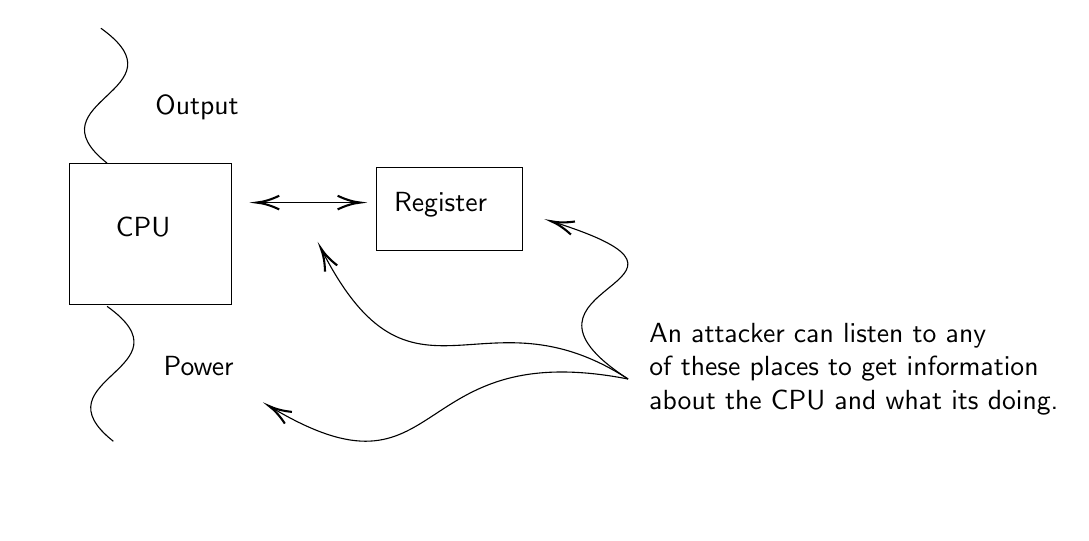
\begin{tikzpicture}[x=0.75pt,y=0.75pt,yscale=-1,xscale=1]
    %uncomment if require: \path (0,300); %set diagram left start at 0, and has height of 300

    %Shape: Rectangle [id:dp8534796086773884] 
    \draw   (54,48) -- (132,48) -- (132,116) -- (54,116) -- cycle ;
    %Straight Lines [id:da5389936541374795] 
    \draw    (144,67) -- (192,67) ;
    \draw [shift={(194,67)}, rotate = 180] [color={rgb, 255:red, 0; green, 0; blue, 0 }  ][line width=0.75]    (10.93,-3.29) .. controls (6.95,-1.4) and (3.31,-0.3) .. (0,0) .. controls (3.31,0.3) and (6.95,1.4) .. (10.93,3.29)   ;
    %Straight Lines [id:da7920000997106575] 
    \draw    (194,67) -- (146,67) ;
    \draw [shift={(144,67)}, rotate = 360] [color={rgb, 255:red, 0; green, 0; blue, 0 }  ][line width=0.75]    (10.93,-3.29) .. controls (6.95,-1.4) and (3.31,-0.3) .. (0,0) .. controls (3.31,0.3) and (6.95,1.4) .. (10.93,3.29)   ;
    %Shape: Rectangle [id:dp1417579616570256] 
    \draw   (202,50) -- (272,50) -- (272,90) -- (202,90) -- cycle ;
    %Curve Lines [id:da37713828096168434] 
    \draw    (72,117) .. controls (114,147) and (37,152) .. (75,182) ;
    %Curve Lines [id:da8627728649790019] 
    \draw    (69,-17) .. controls (111,13) and (34,18) .. (72,48) ;
    %Curve Lines [id:da37559780446173396] 
    \draw    (323,152) .. controls (252.35,106.23) and (219.33,175.3) .. (175.66,90.29) ;
    \draw [shift={(175,89)}, rotate = 423.16999999999996] [color={rgb, 255:red, 0; green, 0; blue, 0 }  ][line width=0.75]    (10.93,-3.29) .. controls (6.95,-1.4) and (3.31,-0.3) .. (0,0) .. controls (3.31,0.3) and (6.95,1.4) .. (10.93,3.29)   ;
    %Curve Lines [id:da7467892221921704] 
    \draw    (323,152) .. controls (252.35,106.23) and (380.71,106) .. (287.42,76.45) ;
    \draw [shift={(286,76)}, rotate = 377.35] [color={rgb, 255:red, 0; green, 0; blue, 0 }  ][line width=0.75]    (10.93,-3.29) .. controls (6.95,-1.4) and (3.31,-0.3) .. (0,0) .. controls (3.31,0.3) and (6.95,1.4) .. (10.93,3.29)   ;
    %Curve Lines [id:da5918015299522423] 
    \draw    (323,152) .. controls (215.54,131.1) and (235.79,216.14) .. (151.28,165.77) ;
    \draw [shift={(150,165)}, rotate = 391.15999999999997] [color={rgb, 255:red, 0; green, 0; blue, 0 }  ][line width=0.75]    (10.93,-3.29) .. controls (6.95,-1.4) and (3.31,-0.3) .. (0,0) .. controls (3.31,0.3) and (6.95,1.4) .. (10.93,3.29)   ;

    % Text Node
    \draw (75,73) node [anchor=north west][inner sep=0.75pt]   [align=left] {CPU};
    % Text Node
    \draw (209,61) node [anchor=north west][inner sep=0.75pt]   [align=left] {Register};
    % Text Node
    \draw (98,140) node [anchor=north west][inner sep=0.75pt]   [align=left] {Power};
    % Text Node
    \draw (94,14) node [anchor=north west][inner sep=0.75pt]   [align=left] {Output};
    % Text Node
    \draw (332,124) node [anchor=north west][inner sep=0.75pt]   [align=left] {An attacker can listen to any\\of these places to get information\\about the CPU and what its doing.};


\end{tikzpicture}


\end{document}